%%% Local Variables:
%%% TeX-command-extra-options: "-shell-escape"
%%% mode: latex
%%% TeX-master: t
%%% End:
\documentclass{beamer}
%\usepackage{listings}
\usepackage{caption}
\usepackage{minted}
\usepackage[labelformat=simple]{subcaption}

\usetheme{Singapore}
\title{Functional Programming}
\subtitle{in Racket}
\author{Peter Campora}
\institute{ULL}
%\date{\today}

\begin{document}
\begin{frame}
\titlepage
\end{frame}

\begin{frame}
  \frametitle{Why Functional Programming?}
  \begin{figure}[t]
    \centering 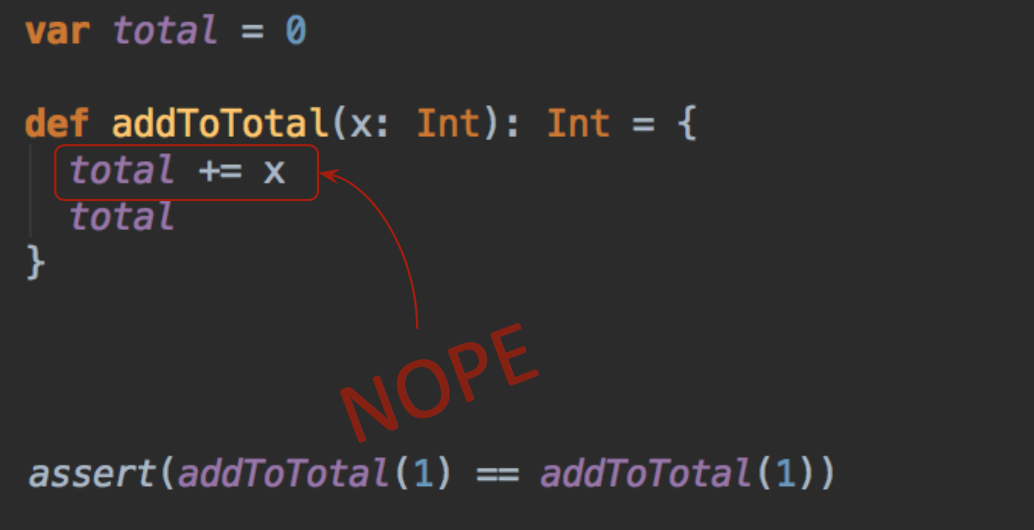
\includegraphics[width=0.3\textwidth]{images/referential-transparency.png}
  \end{figure}
  \begin{itemize}
  \item<2-> The function above isn't \emph{referentially transparent}
  \item<3-> Which means it really isn't even a function in the \emph{mathematical} sense.
  \item<4-> This makes it hard to create reproducible behavior or prove code correctness
  \item<5-> Concurrent programming is made difficult since order of evaluation matters.
  \item<6-> Functional idioms creep into imperative languages. Lambda and streams
    were added to Java, and JavaScript code becomes increasingly functional.
  \end{itemize}
\end{frame}
 
\begin{frame}  
  \frametitle{What Things are Beautiful?}
  \begin{figure}[t]
    \begin{subfigure}[b]{.3\textwidth}
      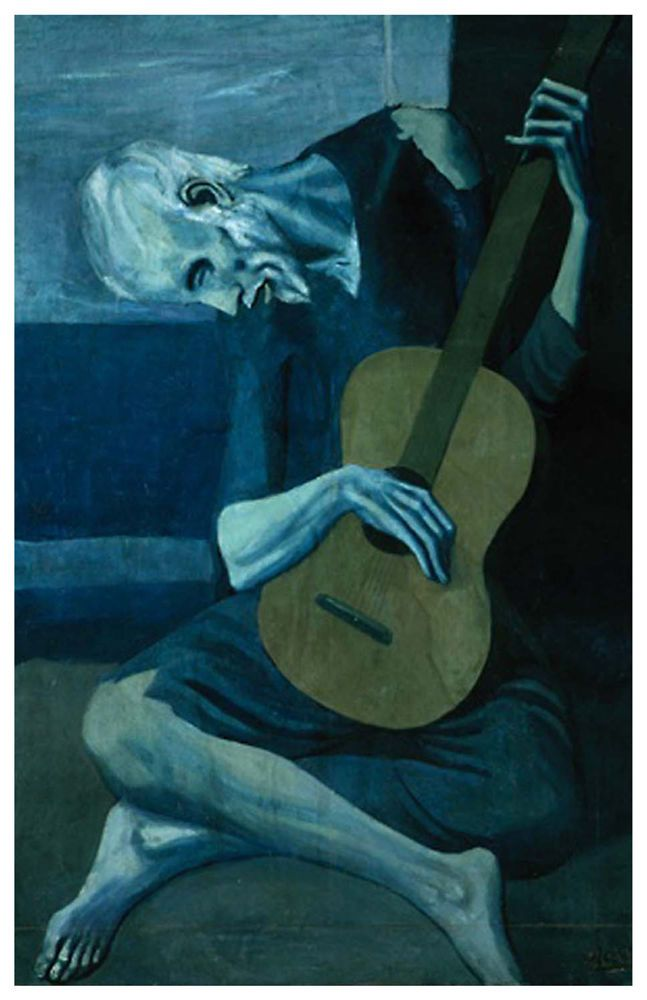
\includegraphics[width=.9\textwidth]{images/old-guitarist.jpg}       
    \end{subfigure}
    \pause
    \begin{subfigure}[b]{.3\textwidth}
      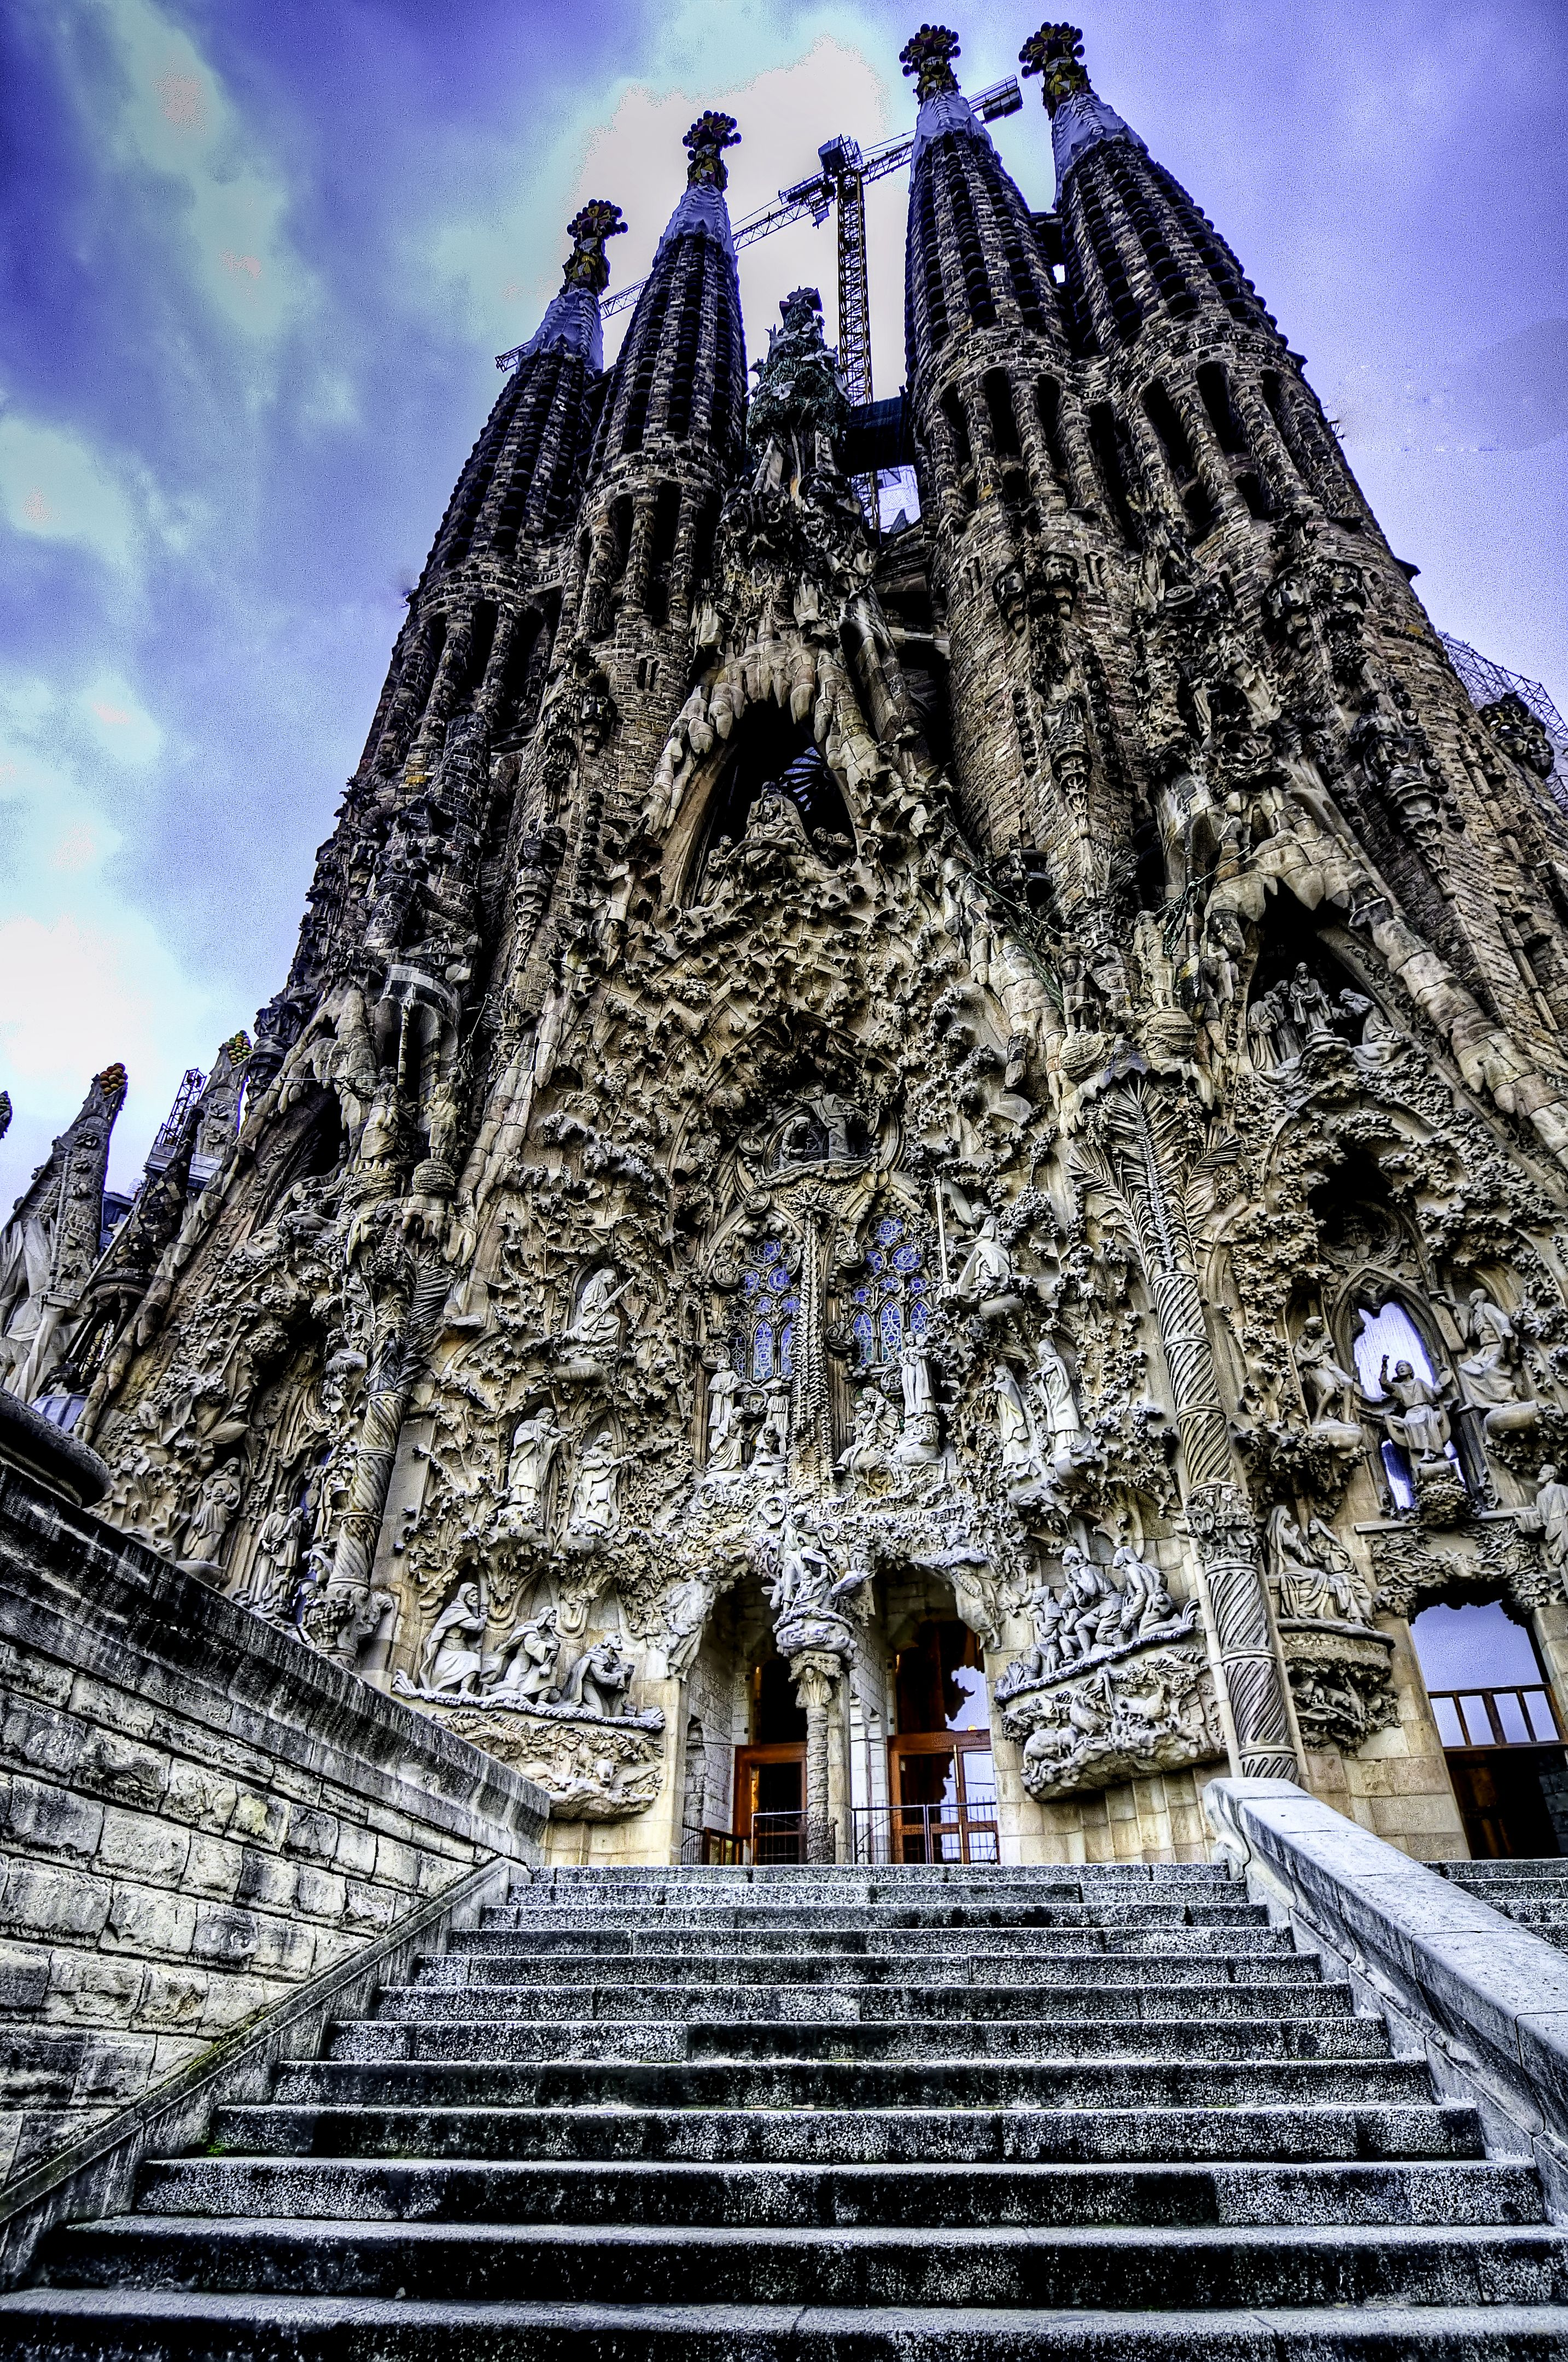
\includegraphics[width=.9\textwidth]{images/sagrada-familia.jpg}
    \end{subfigure}
    \pause
    \begin{subfigure}[b]{.3\textwidth}
      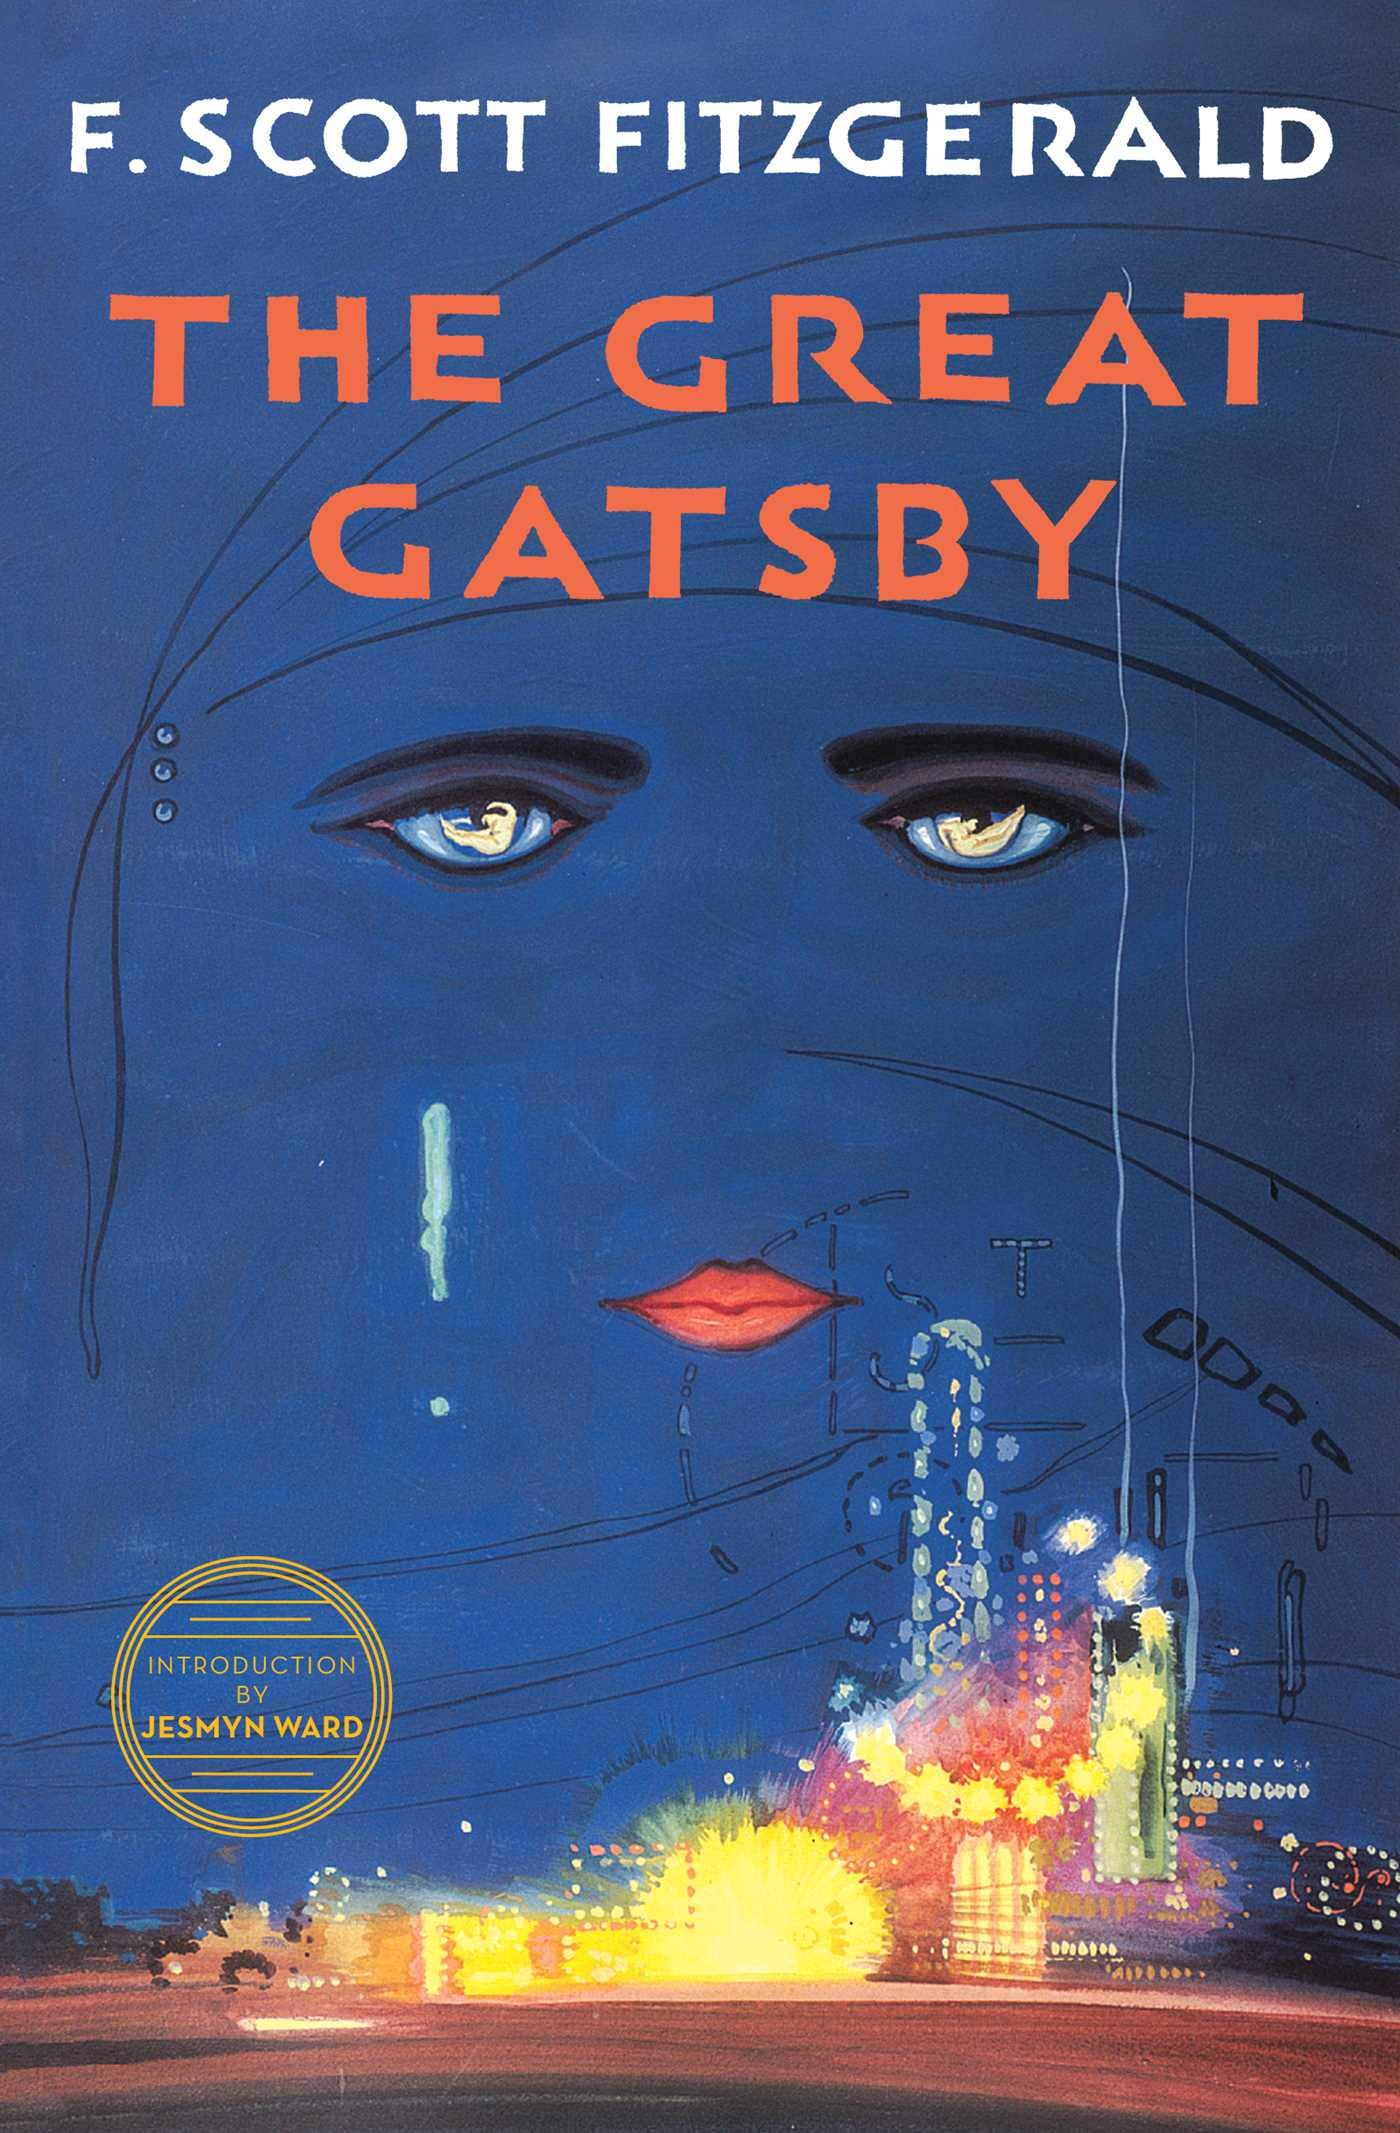
\includegraphics[width=.9\textwidth]{images/great-gatsby.jpg}
    \end{subfigure}   
  \end{figure}
% \begin{itemize}
% \item Suitable for a Specific Problem Domain or Platform
% \item Point B
% \begin{itemize}
% \item part 1
% \item part 2
% \end{itemize}
% \item Point C
% \item Point D
% \end{itemize}
\end{frame}

% \defverbatim[colored]\lstI{
%   \begin{lstlisting}[language=Java,basicstyle=\ttfamily,keywordstyle=\color{blue},stringstyle=\color{red}\ttfamily,
%            commentstyle=\color{green}\ttfamily,breaklines=True]
% public class SumSquares
% {
%    public static void main(final int[] nums)
%    {
%       int sum = 0;      
%       for (int i : nums)
%         sum += i * i;
%       System.out.println("The sum of the squares is: " + sum);
%     }
% }    
%   \end{lstlisting}
% }
\defverbatim[colored]\lstI{
  \begin{minted}[breaklines]{Java}
public class SumSquares
{
   public static void main(final int[] nums)
   {
      int sum = 0;      
      for (int i : nums)
        sum += i * i;
      System.out.println("The sum of the squares is: " + sum);
    }
}    
\end{minted}
}
\begin{frame}
  \frametitle{Can Code be Beautiful?}
  Write a program for summing the squares of numbers from 1 to n.
  \pause
    \lstI
\end{frame}

\defverbatim[colored]\lstR{
\begin{minted}{racket}
;;Number -> Number
(define (square x) (* x x))

;;Number List -> Number List
(define (sum-of-squares lst)
  (sum (map square lst))         
\end{minted}
}

\begin{frame}
  \frametitle{An Equivalent Program}
  Let's get our first look at a functional program written in Racket.
  \pause
  \lstR
  \pause
  Don't worry about the meaning and syntax of the program, yet.
  Given time, the parens will become beautiful!
\end{frame}

\begin{frame}
  \frametitle{What \emph{Is} Code Beauty?}
  First let's hear from you!
  \pause
  Let's consider some other views.
  \begin{itemize}
  \item<2-> Utilitarian Program Beauty 
    \begin{itemize}
    \item<3-> The programming language that maximizes the utility of writing my program is the best. Minimize bugs, execution time, and time until production.
    \item<4-> Critique: Hard to measure which features objectively help the process of writing programs.
    \end{itemize}
  \item<5-> Egoist Program Beauty 
    \begin{itemize}
    \item<6-> The programming language that allows me to write clever, expressive programs is best. 
    \item<7-> Critique: Engineering is largely a social endeavor. Other people need to be able to read your programs and understand abstractions.
    \end{itemize}
  \item<8-> Aesthetic Program Beauty 
    \begin{itemize}
    \item<9-> Beauty is subjective according to appreciation of the idioms of some paradigm (i.e. cubism in art).
    \item<10-> Critique: Disconnected from the empirical or mathematical viewpoints we typically employ to measure the value of scientific contributions. 
    \end{itemize}
  \end{itemize}
\end{frame}

\begin{frame}
  \frametitle{Looks Like We Don't Know}
  \begin{figure}
    \centering
    
\includegraphics[width=.7\textwidth]{images/mr-krabs.jpeg}
  \end{figure}
\end{frame}

\begin{frame}
  \frametitle{So, Why Ask?}
  \begin{itemize}
  \item<1-> Universities are a place for the creation and acquisition of knowledge.
  \item<2-> We should put our opinions under scrutiny.
  \item<3-> Computer Scientists are critical thinkers.
  \end{itemize}
\end{frame}

\begin{frame}
  \frametitle{How Do We Write Programs?}
  \begin{figure}
    \begin{subfigure}[b]{0.4\textwidth}
      
\includegraphics[width=0.9\textwidth]{images/staring-at-a-blank-wall.jpg}
    \end{subfigure}
    \pause
    \begin{subfigure}[b]{0.4\textwidth}
      
\includegraphics[width=0.8\textwidth]{images/eureka.jpg}
    \end{subfigure}
  \end{figure}
\end{frame}

\begin{frame}
  \begin{center}
    \huge Let's hear from you.
  \end{center}
\end{frame}

\begin{frame}
  \frametitle{Is Programming Hard?}
  \begin{figure}[t]
    \begin{subfigure}[b]{0.3\textwidth}
      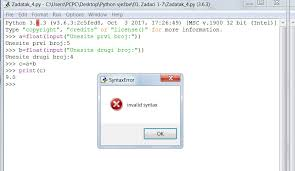
\includegraphics[width=0.9\textwidth]{images/syntax-error.jpeg}
    \end{subfigure}
    \pause
    \begin{subfigure}[b]{0.3\textwidth}
      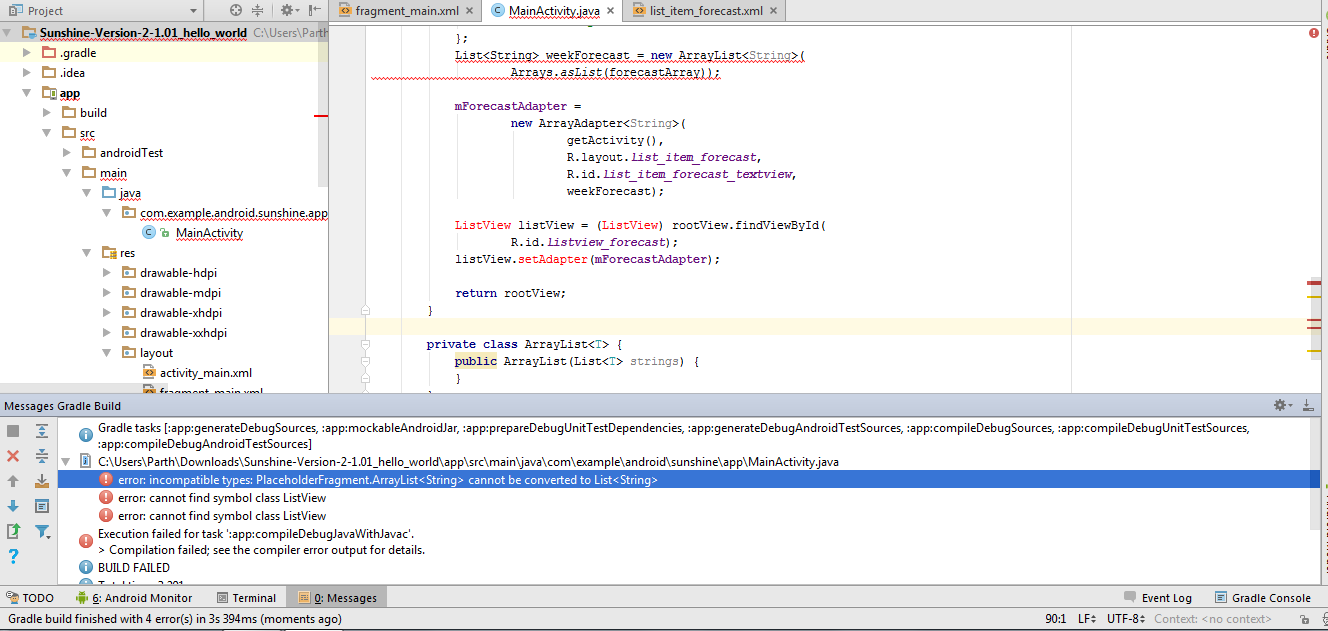
\includegraphics[width=0.8\textwidth]{images/type-error.png}
    \end{subfigure}
    \pause
    \begin{subfigure}[b]{0.3\textwidth}
      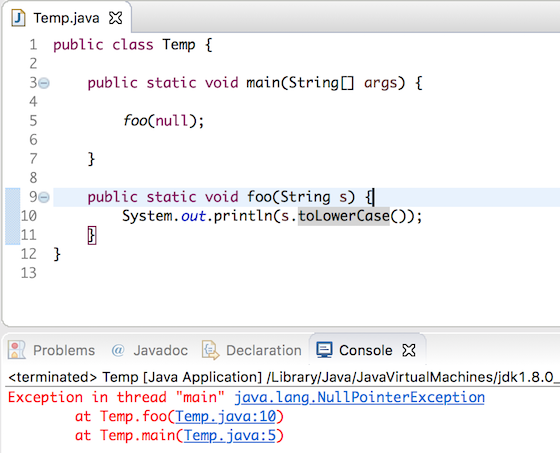
\includegraphics[width=0.8\textwidth]{images/nullpointerexception.png}
    \end{subfigure}
  \end{figure}
  \pause
  \begin{figure}
    \begin{subfigure}[t]{0.3\textwidth}
      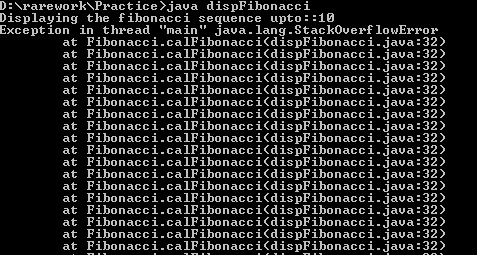
\includegraphics[width=0.9\textwidth]{images/stack-overflow.png}
    \end{subfigure}
    \pause
    \begin{subfigure}[t]{0.3\textwidth}
      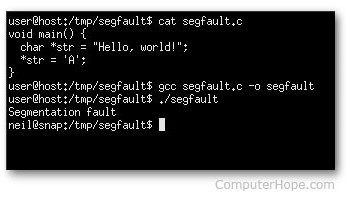
\includegraphics[width=0.8\textwidth]{images/segfault.jpg}
    \end{subfigure}
    \pause
    \begin{subfigure}[t]{0.3\textwidth}
      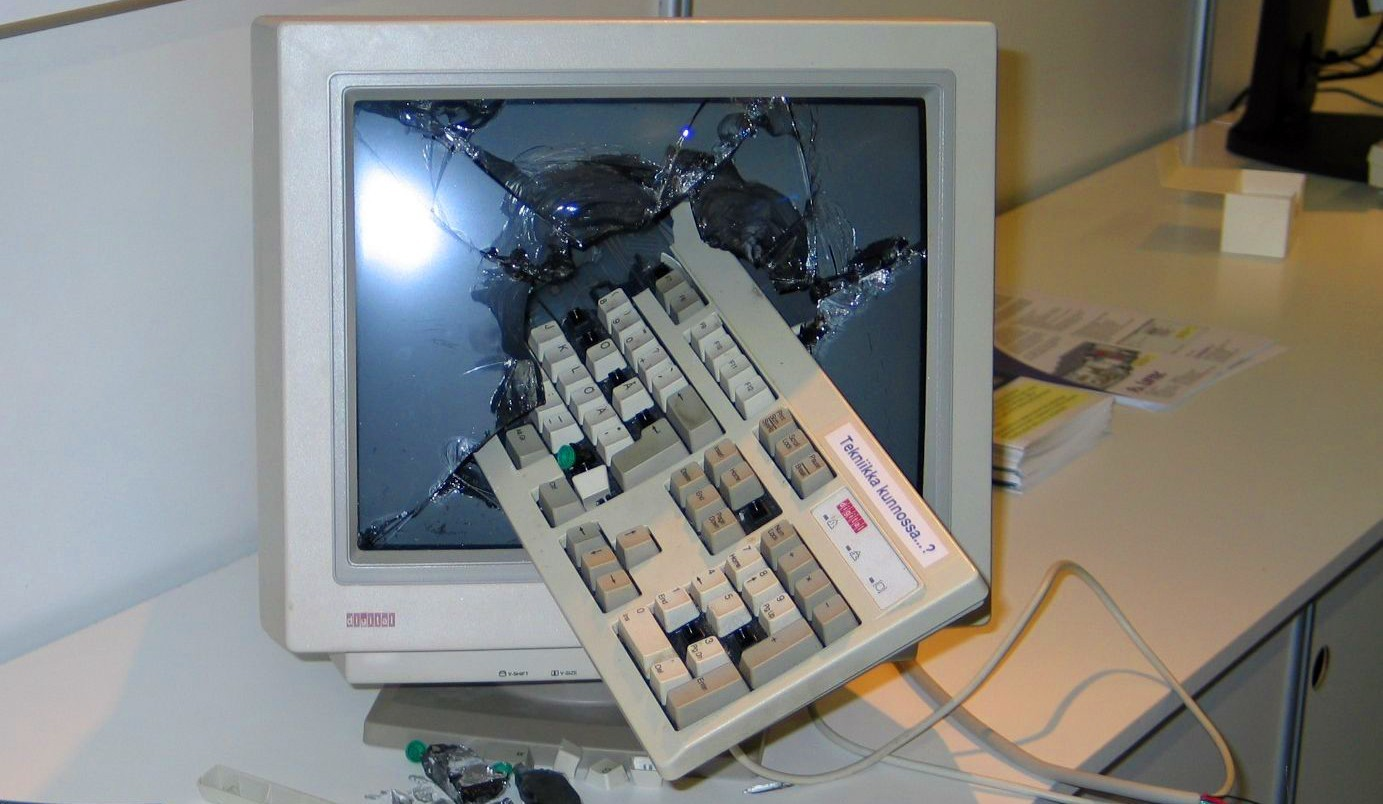
\includegraphics[width=0.8\textwidth]{images/break-computer.jpg}
    \end{subfigure}
  \end{figure}
\end{frame}

\begin{frame}
  \frametitle{How Programming Is Taught}
  \begin{figure}[t]
    \centering 
\includegraphics[width=0.3\textwidth]{images/pattern-recognition.jpg}
  \end{figure}
  \begin{itemize}
  \item<2-> Programming courses typically start by motivating new features with concrete programs.
  \item<3-> Given enough examples, students begin to match problem descriptions to using features.
  \item<4-> From there, programming becomes gluing together recognized patterns.
  \item<5-> \textbf{There has to be a better way!}
  \end{itemize}
\end{frame}

\begin{frame}
  \frametitle{The Better Way}
  \begin{figure}[t]
    \centering 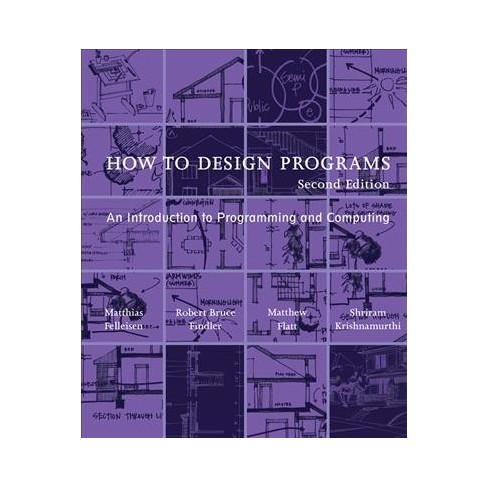
\includegraphics[width=0.3\textwidth]{images/htdp.jpeg}    
  \end{figure}
  \begin{itemize}
  \item<2-> This book (and course) will teach systematic program design.
  \item<3-> It presents recipes for designing two different types of programs.
    \begin{itemize}
    \item<4-> Big bang (event driven) programs
    \item<5-> Batch programs (effectful scripts)
    \end{itemize}
  \item<6-> Isn't this a course on functional programming?    
  \end{itemize}
\end{frame}

\begin{frame}
  \frametitle{Learning Functional Programming from the Ground Up}
  \begin{figure}[t]
    \centering 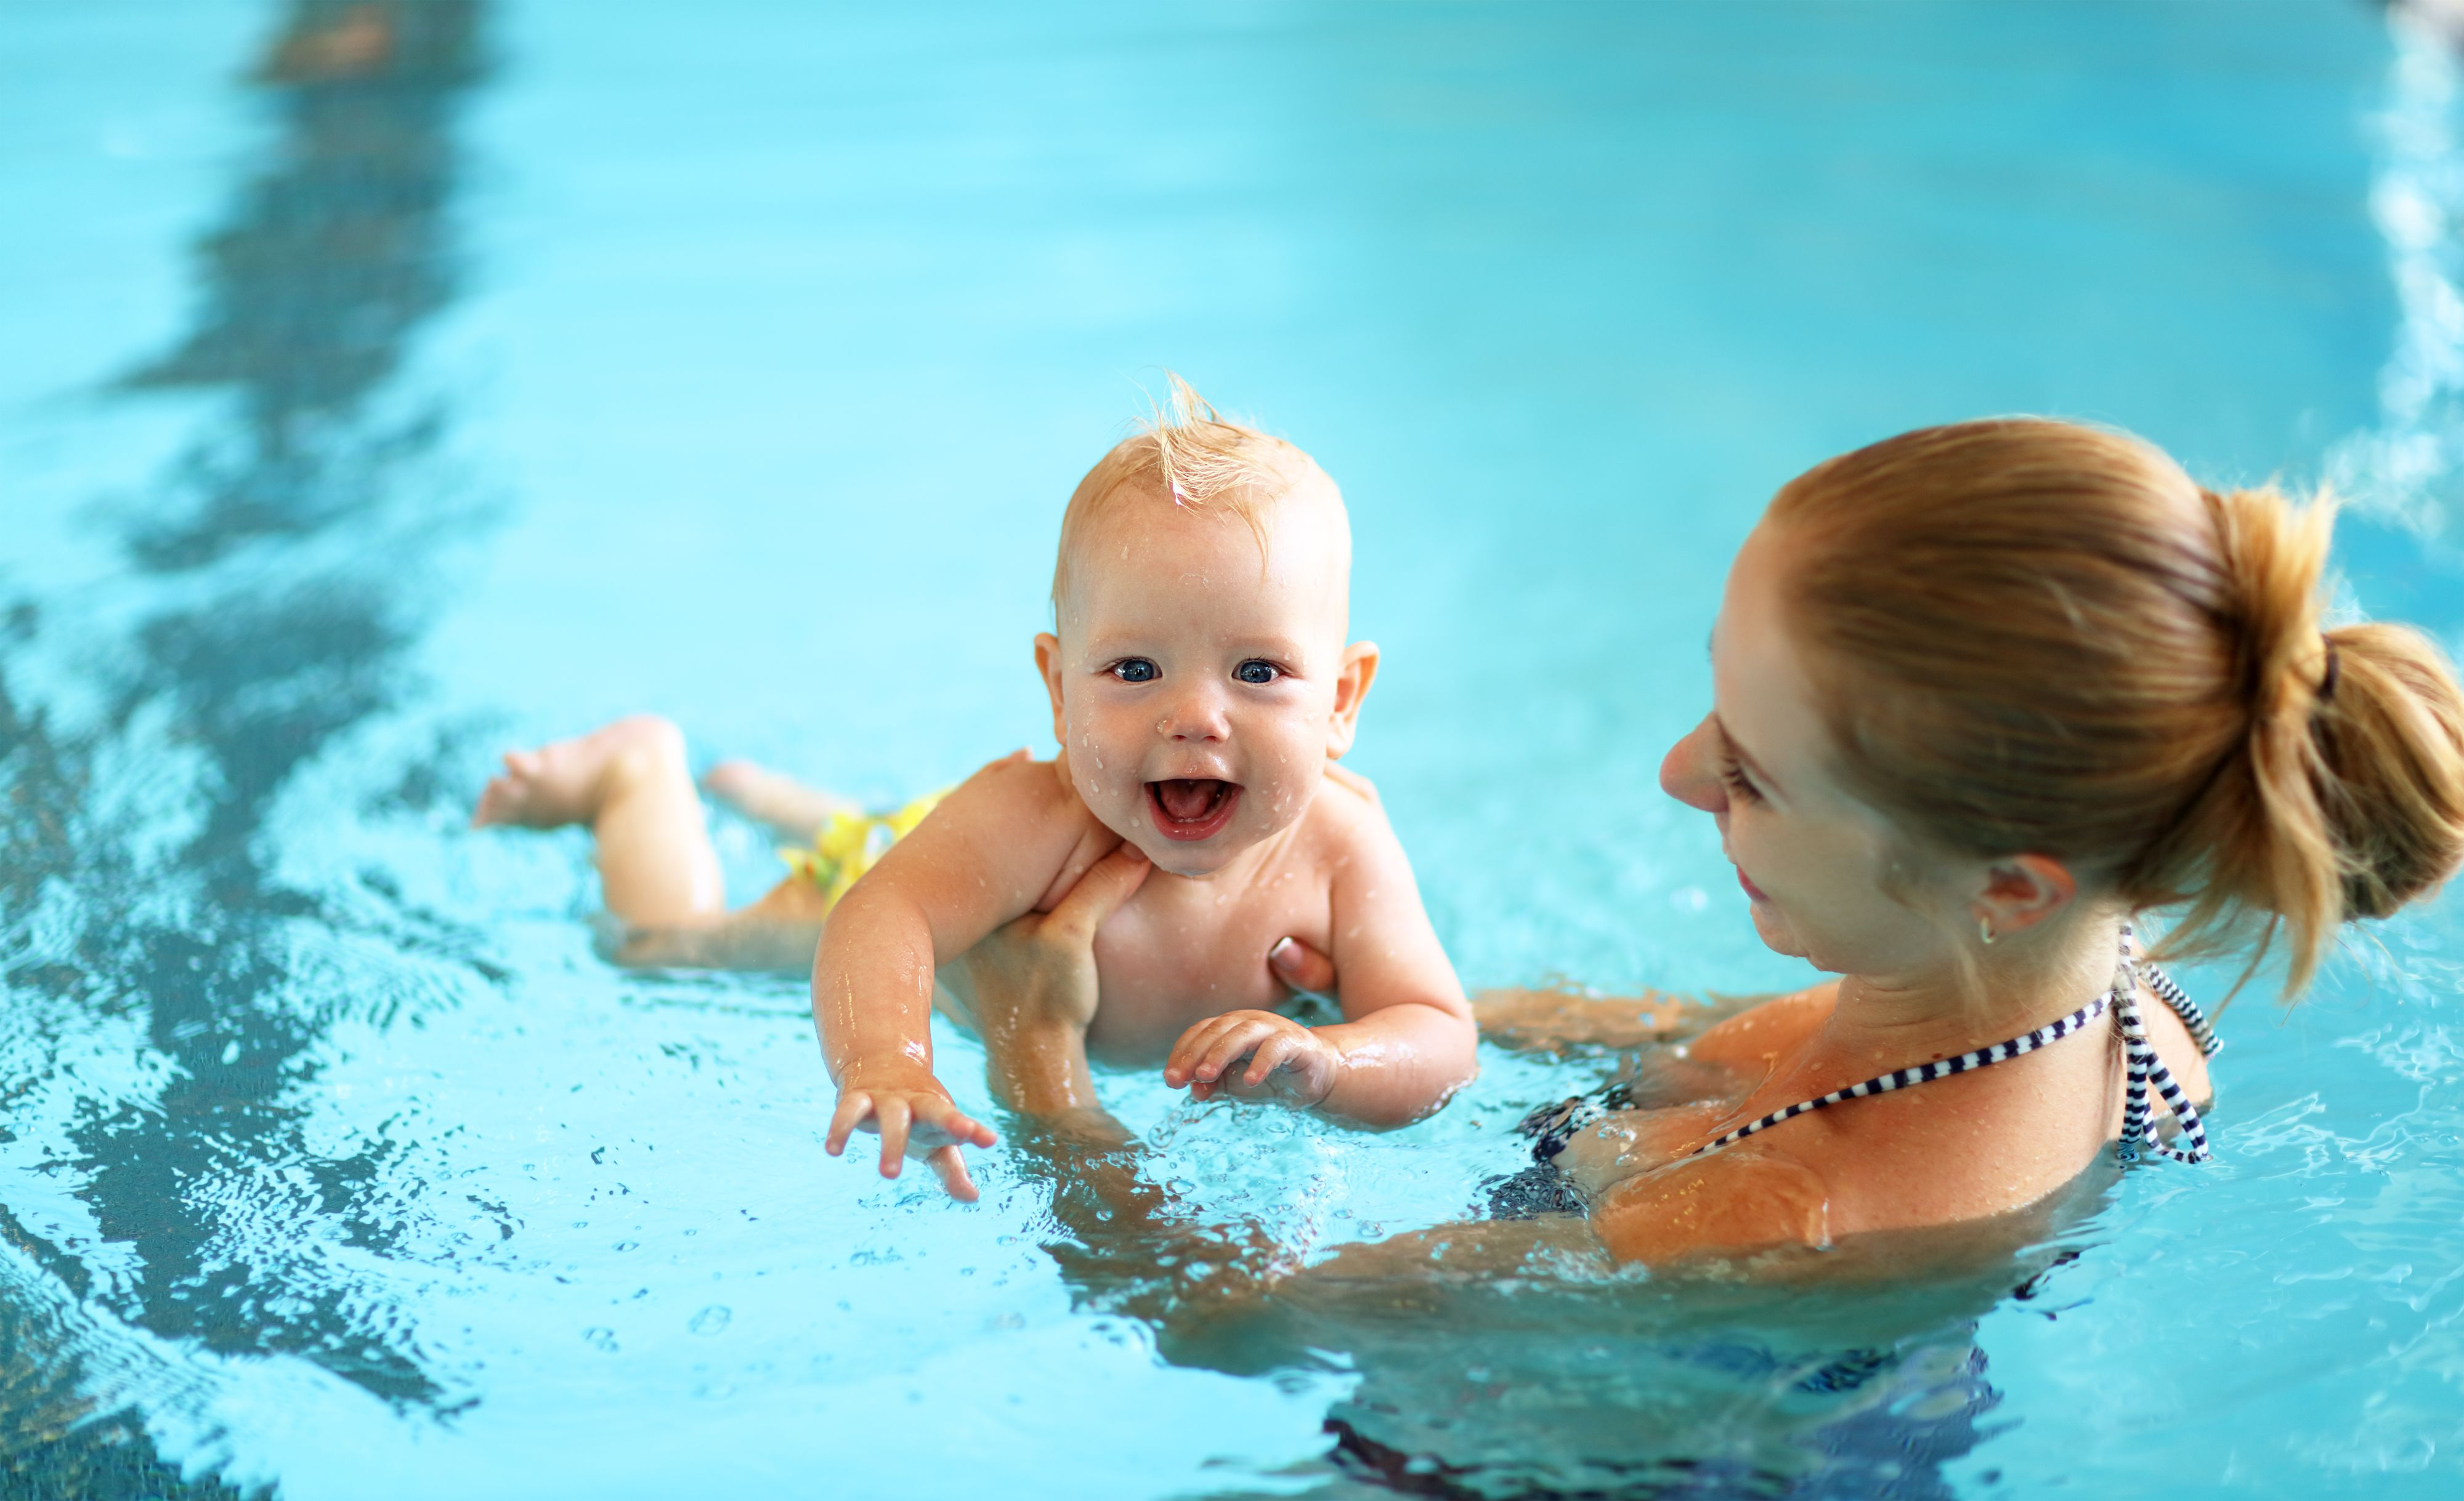
\includegraphics[width=0.3\textwidth]{images/pool-baby.jpeg}
  \end{figure}
  \begin{itemize}
  \item<2-> Why How to Design Programs?
  \item<3-> When I first tried to learn functional programming, I failed.
  \item<4-> 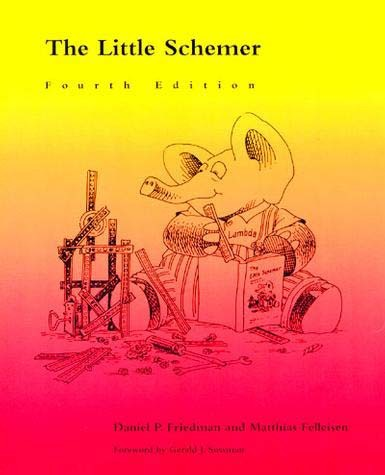
\includegraphics[width=0.2\textwidth]{images/little-schemer.jpg}
  \item<5-> We will learn functional programming and systematic design, together!
  \end{itemize}  
\end{frame}

\begin{frame}
  \frametitle{Why Racket and Not X?}
  \begin{figure}[t]
    \centering 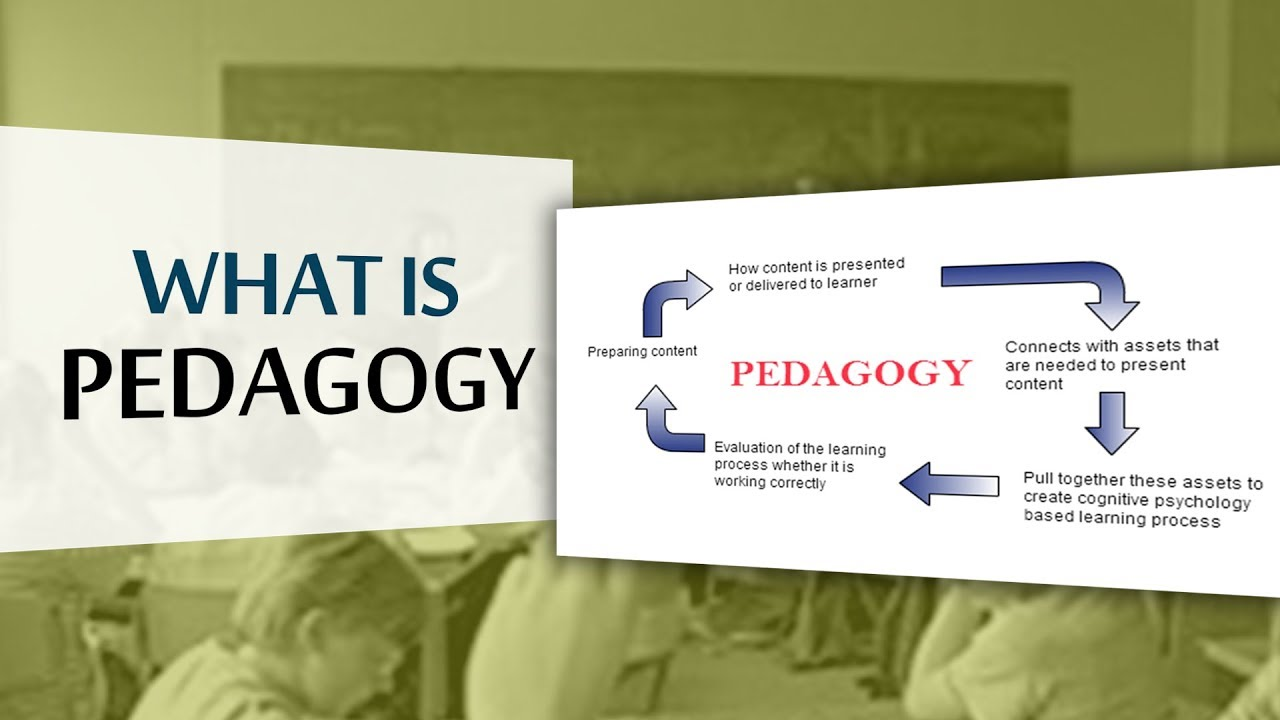
\includegraphics[width=0.3\textwidth]{images/pedagogy.jpg}
  \end{figure}
  \begin{itemize}
    \item<2-> Teaching functional programming in an imperative-first language is awkward
    \item<3-> Other functional languages have additional complexity
    \item<4-> It's focused on being a good language for education
  \end{itemize}
\end{frame}

\begin{frame}
  \frametitle{Course Structure}
  Grades will come from:
  \begin{itemize}
  \item<1-> Programming assignments (can be done as a team of up to 5 people)
  \item<2-> 4-6 projects (individual but last project as a team)    
  \item<3-> An easy test and final    
  \item<4-> \emph{Try not to stress about grades and \emph{don't cheat}}
  \item<5-> I don't want to use this:
    \begin{figure}[t]
      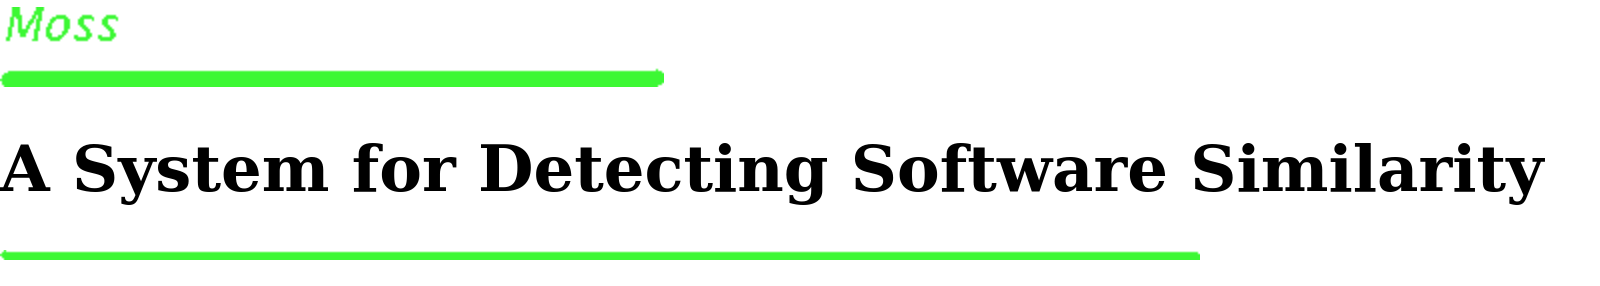
\includegraphics[width=0.6\textwidth]{images/moss.png}
    \end{figure}
  \end{itemize}
\end{frame}

\begin{frame}
  \frametitle{The Main Things I Want}
  \begin{figure}[t]
    \begin{subfigure}{0.45\textwidth}
      
\includegraphics[width=0.9\textwidth]{images/think-different.jpg}
    \end{subfigure}
    %
    \begin{subfigure}{0.45\textwidth}
      
\includegraphics[width=0.95\textwidth]{images/brain.jpg}
    \end{subfigure}
  \end{figure}
  
\end{frame}

\begin{frame}
  \begin{center}
    \huge What do you want?
  \end{center}
\end{frame}

% \begin{frame}
%   \frametitle{Course Outcomes}
%   \begin{itemize}
%   \item<1-> Learn systematic program design recipes and how to iteratively refine programs
%   \item<2-> Get comfortable with concepts like higher-order functions
%   \item<3-> Get comfortable with writing recursive programs and dealing with inductive data
%   \item<4-> Learn how data input and output leads the design of programs
%   \item<5-> Use functional idioms in imperative/OO languages like Java and Python
%   \item<6-> 
%   \end{itemize}
\end{document}
%%% Local Variables:
%%% TeX-command-extra-options: "-shell-escape"
%%% mode: latex
%%% TeX-master: t
%%% End:
